Veamos los siguientes sistemas:

\begin{equation}
    G(s) = \frac{3s + 9}{s^3 + 11s^2 + 19.25s + 92.5} \qquad H(s) = \frac{2(s+5)}{(s+2)(s+4)^2}
\end{equation}



Utilizando los comandos \texttt{zeros, pole} y \texttt{pzmap}, podemos calcular los ceros, polos y graficarlos respectivamente. El siguiente código muestra cómo hacerlo y el resultado, también la gráfica obtenida de los polos y ceros (\ref{fig:1}).

\begin{lstlisting}
clear all
close all
clc

%Sistemas
Gs = tf([3, 9], [1, 11, 19.25, 92.5]);
Hs = zpk([-5], [-2, -4, -4], 2);

%ceros
Gs_ceros = zero(Gs);
>> -3
Hs_ceros = zero(Hs);
>> -5

%polos
Gs_polos = pole(Gs);
>> -10 + 0i
   -0.5 + 3i
   -0.5 - 3i 
Hs_polos = pole(Hs);
>> -2
   -4
   -4

%Graficos
fig = figure;
theme(fig, "light");
pzmap(Gs);
hold on;
pzmap(Hs);
\end{lstlisting}


\begin{figure}[ht!]
    \centering
    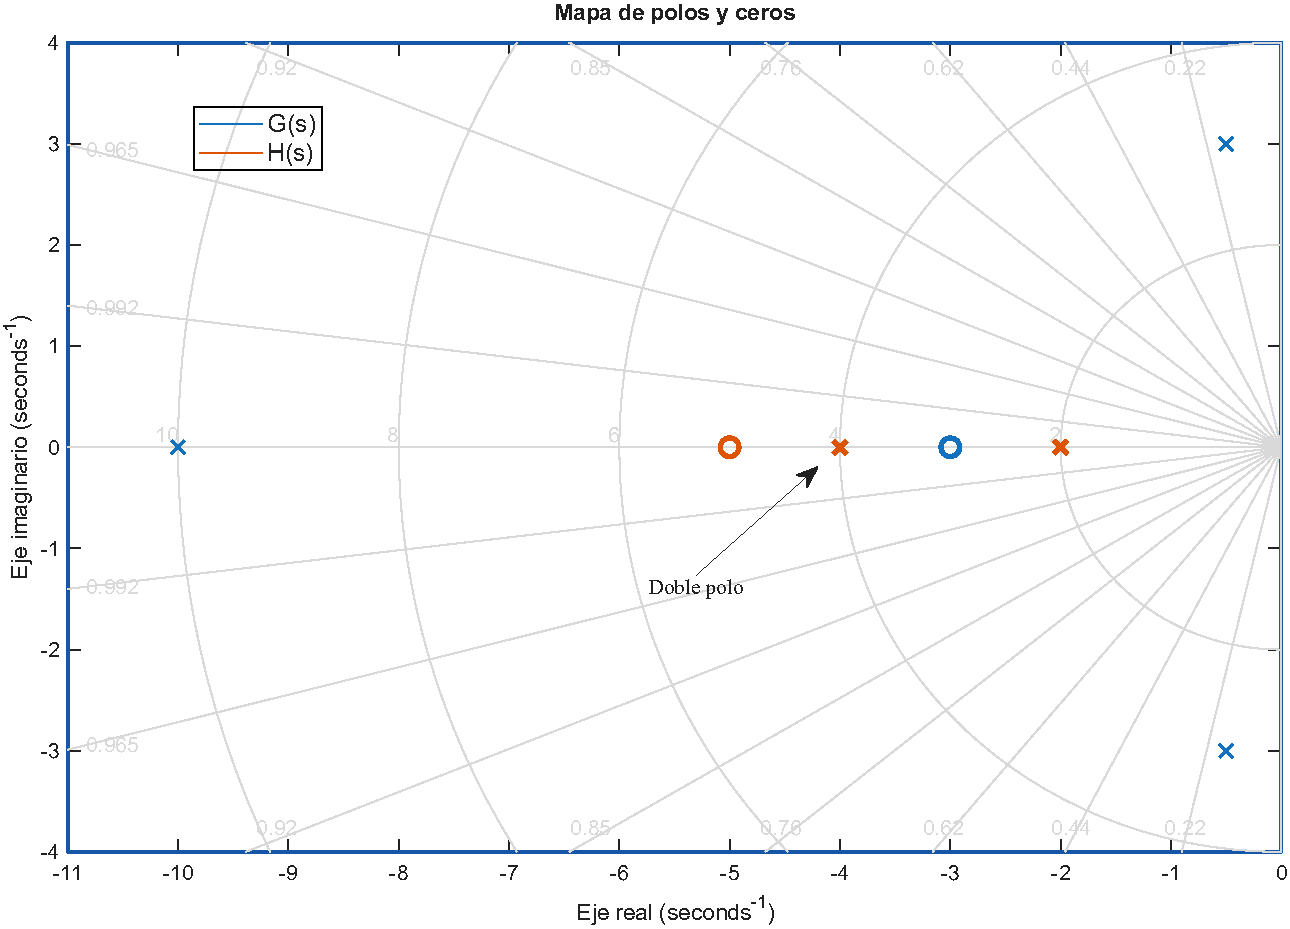
\includegraphics[width=0.6\textwidth]{imagenes/mapa_polos_y_ceros.pdf}
    \caption{Gráfico de los polos y ceros de $G(s)$ y $H(s)$}
    \label{fig:1}
\end{figure}


De la figura \ref{fig:1} podemos concluir que el sistema $G(s)$ tendrá un sobrepaso del 59.2\%, mientras que $H(s)$ no lo tiene.


También podemos construir un nuevo sistema $C_1$, donde $H$ es el compensador de $G$, mediante la forma \texttt{C1 = feedback(Gs, Hs)}.

Observemos la siguiente figura:

\begin{figure}[htbp]
    \centering
    \begin{tikzpicture}[
        line width=0.8pt,
        bloque/.style={
            draw,
            rectangle,
            minimum width=1.4cm,
            minimum height=0.8cm
        },
        sumador/.style={
            draw,
            circle,
            fill=white,
            minimum size=2mm,
            inner sep=0pt
        }
    ]

        % Recuadro que contiene el sistema C_2.
        \draw[
            dashed,
            rounded corners=10pt,
            line width=0.6pt
        ] (-1.0,-1.5) rectangle (5.4,0.7);

        \node[anchor=west] at (-0.7,-1.15) {$C_2$};

        % Bloques y sumador.
        \node[bloque]  (H)    at (0,0)   {$H(s)$};
        \node[sumador] (suma) at (1.9,0) {};
        \node[bloque]  (G)    at (3.8,0) {$G(s)$};

        % Punto de donde sale la realimentación.
        \coordinate (retorno) at (5.1,0);

        % Entrada.
        \draw[-Latex] (-1.8,0)
            -- node[above, pos=0.2] {$R(s)$} (H.west);

        % Conexiones entre los bloques.
        \draw[-Latex] (H.east)
            -- node[above] {$u$} (suma.west);

        \draw[-Latex] (suma.east)
            -- node[above] {$e$} (G.west);

        % Salida.
        \draw[-Latex] (G.east)
            -- (6.1,0) node[above] {$Y(s)$};

        % Realimentación negativa.
        \draw[-Latex] (retorno)
            -- (5.1,-1.15)
            -| (suma.south);

        % Signo junto a la entrada inferior del sumador.
        \node at (2.12,-0.25) {$-$};

    \end{tikzpicture}

    \caption{Diagrama de bloques del sistema $C_2$.}
    \label{fig:diagrama-c2}
\end{figure}



Podemos implementar el sistema $C_2$ mediante la función \texttt{connect}. La misma nos dará la función de transferencia según la entrada y salida solicitada. El siguiente código y gráfico muestra cómo implementar la función connect, así como la gráfica del sistema $C_2$, $H$ y $G$ mediante una entrada impulso y entrada (figura \ref{fig:2}).

\begin{lstlisting}
%Uso del connect

%Primer sistema
Hs.InputName = 'r';
Hs.OutputName = 'u';
Gs.InputName = 'e';
Gs.OutputName = 'y';
Sum = sumblk('e = u - y');
sys1 = feedback(Gs, 1);

C2 = connect(Hs, sys1, Sum, 'r', 'y');

%Entrada escalon
tiledlayout(2,1);
ax1 = nexttile;
stepplot(ax1, Gs, 'r', Hs, 'b--', C2, 'g');
title(ax1, 'Respuesta escalon')

%Entrada impulso
ax2 = nexttile;
impulseplot(ax2, Gs, 'r', Hs, 'b--', C2, 'g');
title(ax2,  'Respuesta impulso')

%Voy a determinar la info con lsiminfo para el impulso
[yG, tG] = impulse(Gs);
[yH, tH] = impulse(Hs);
[yC2, tC2] = impulse(C2);

info_gs_impulso = lsiminfo(yG, tG, 0);
info_hs_impulso = lsiminfo(yH, tH, 0);
info_c2s_impulso = lsiminfo(yC2, tC2, 0);

\end{lstlisting}


\begin{figure}[ht!]
    \centering
    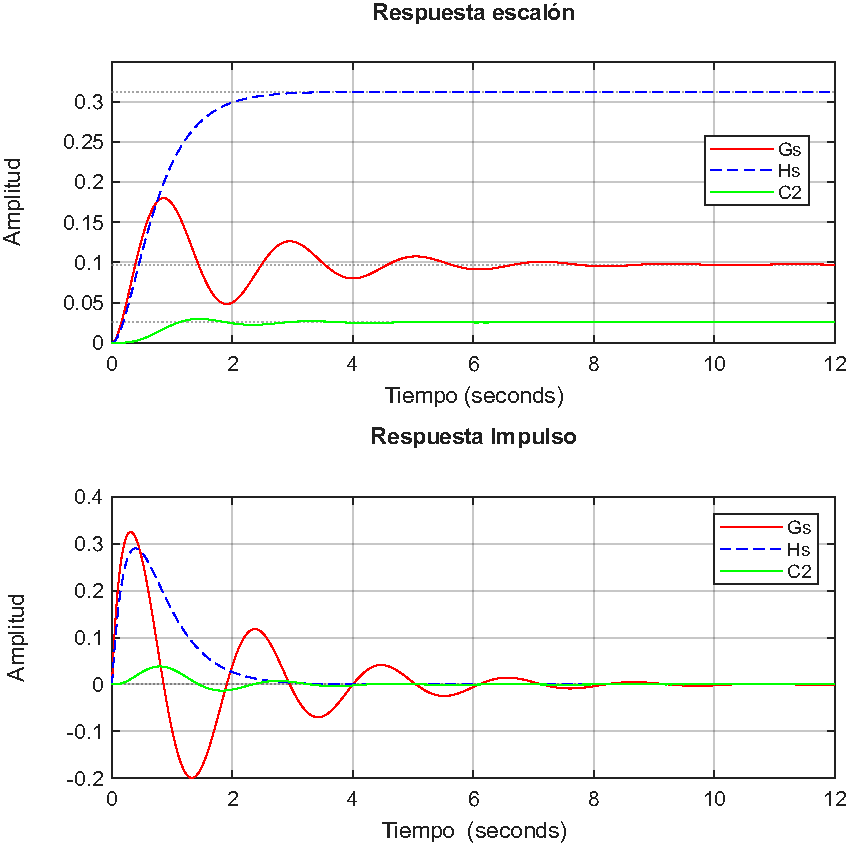
\includegraphics[width=0.8\textwidth]{imagenes/figura_impulso_y_escalon.pdf}
    \caption{Respuesta de los sistemas mediante entradas escalón e impulso}
    \label{fig:2}
\end{figure}




Usando las funciones \texttt{stepinfo} y \texttt{lsiminfo} podemos determinar los valores de \textit{settling times} y \textit{rise times}. En la Tabla \ref{tab:1} se compara los valores de tiempo para cada sistema.

\begin{table}[ht!]
    \centering
    \renewcommand{\arraystretch}{1.3}

    \begin{tabular}{|c|c|c|c|c|}
        \hline

        % Encabezado principal.
        \multirow{2}{*}{\textbf{Sistema}}
        & \multicolumn{2}{c|}{\textbf{Escalón}}
        & \multicolumn{2}{c|}{\textbf{Impulso}} \\
        \cline{2-5}

        % Subcolumnas de cada tipo de respuesta.
        & \shortstack{Settling time (s)}
        & \shortstack{Rise time (s)}
        & \shortstack{Settling time (s)}
        & \shortstack{Rise time (s)} \\
        \hline

        $G(s)$   & 8.3247&0.2665 & 7.853 & - \\
        \hline
        $H(s)$   & 2.388 & 1.354& 2.771&  -\\
        \hline
        $C_2(s)$ & 4.496& 0.614 &5.789 & - \\
        \hline
    \end{tabular}

    \caption{Comparación de los tiempos de asentamiento y de subida
    para las respuestas al escalón y al impulso. Los valores que tienen raya es porque no se encontró una manera de calcular dichos valores.}
    \label{tab:1}
\end{table}


Ahora pasemos a los diagramas de Bode. un diagrama de Bode está formado por dos gráficas: una es la gráfica del logaritmo de la magnitud de la función de transferencia sinusoidal, y la otra es la gráfica del ángulo de fase; ambas se dibujan contra la frecuencia en escala logarítmica. En la figura \ref{fig:3} se grafican los diagramas de bode de las funciones transferencia $G$ y $H$.
De la figura se observa que $G(s)$ presenta un pico en $2.96$ rad/s.

\newpage

\begin{figure}[ht!]
    \centering
    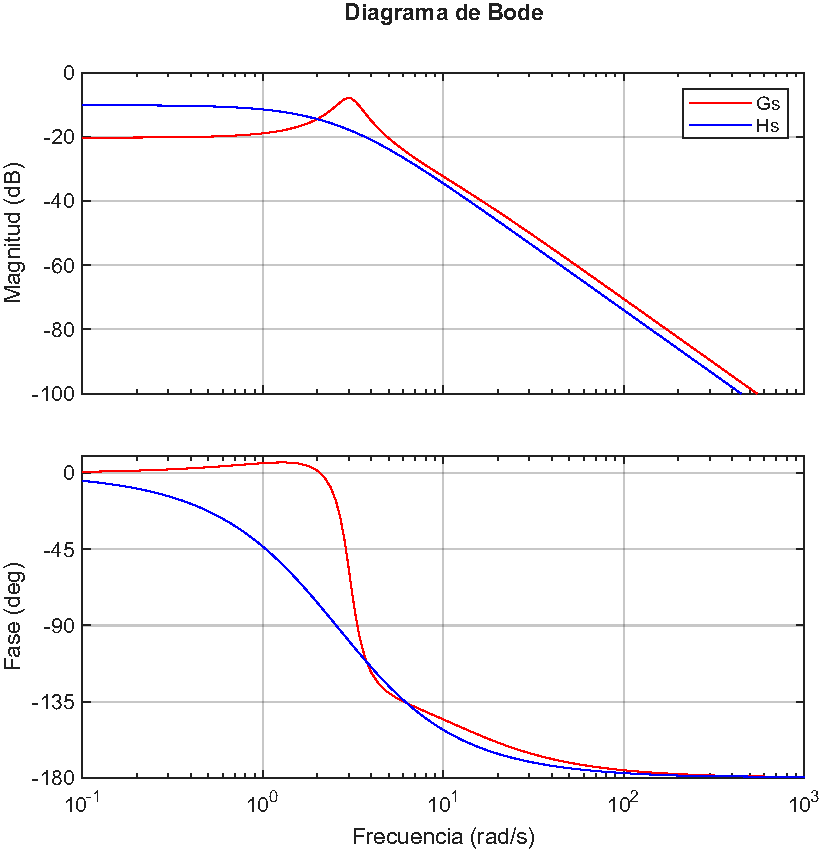
\includegraphics[width=0.65\textwidth]{imagenes/bode_g_y_h.pdf}
    \caption{Diagrama de Bode}
    \label{fig:3}
\end{figure}


Ahora analicemos la siguiente función:

\begin{equation}
    F(s) = \frac{3}{(s+2-9i)(s+2+9i)}
\end{equation}


\noindent y su diagrama de Bode. El pico se encuentra en 8.77 rad/s.

\begin{figure}[ht!]
    \centering
    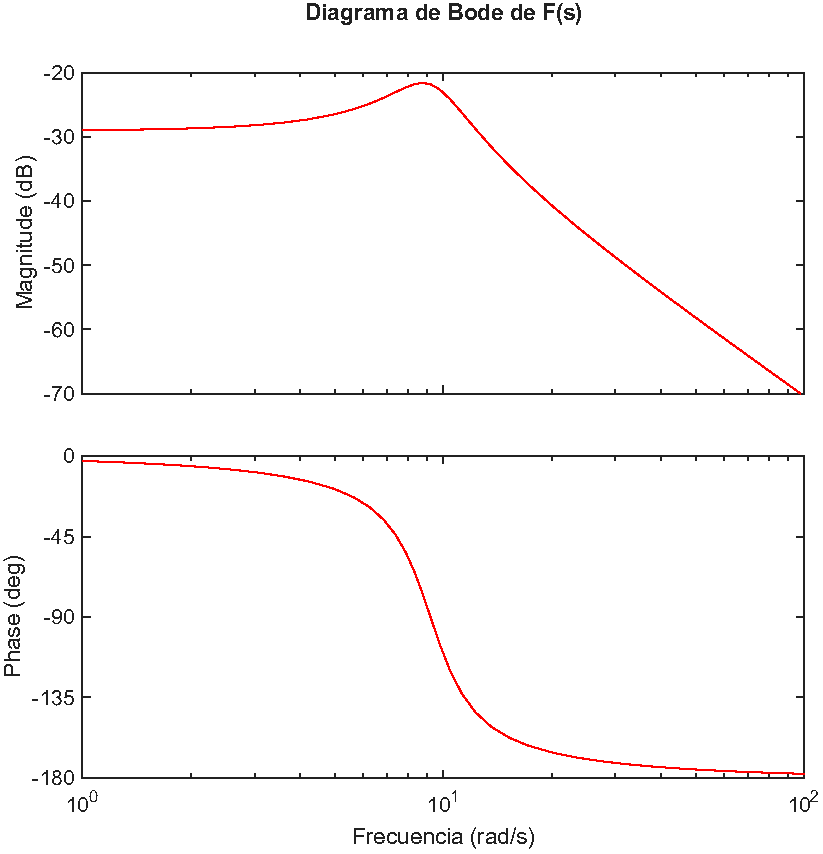
\includegraphics[width=0.65\textwidth]{imagenes/bode_de_f.pdf}
    \caption{Diagrama de bode de $F$}
    \label{fig:4}
\end{figure}




Por último, veamos el diagrama de Nyquist de $G(s)$ y el ancho de banda de $G$ y $H$.


\begin{figure}[ht!]
    \centering
    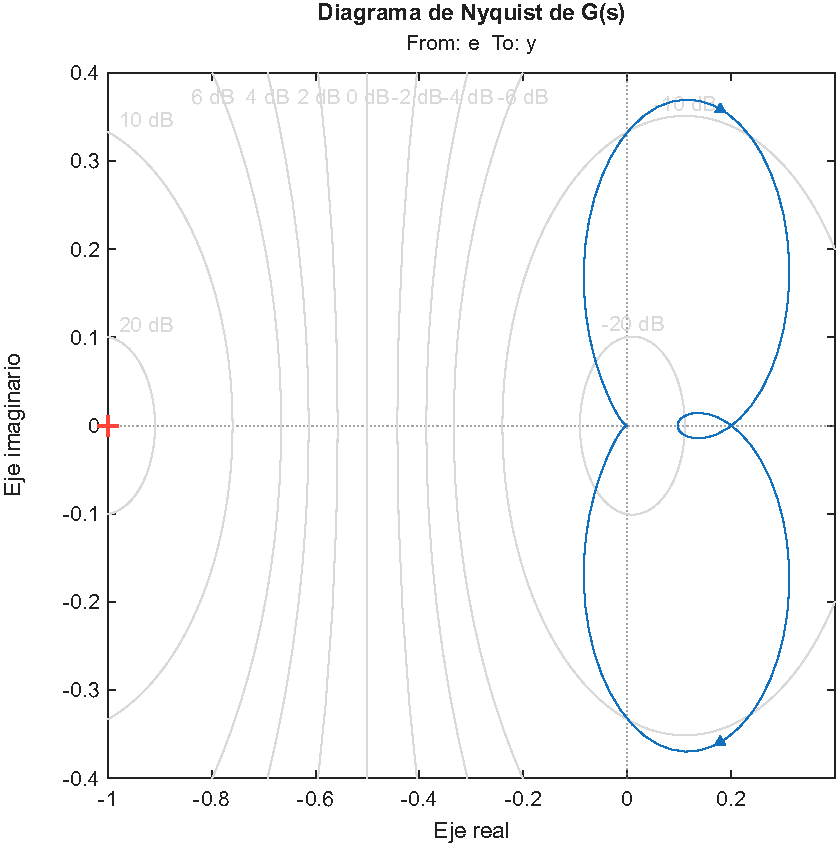
\includegraphics[width=0.7\textwidth]{imagenes/nyquist.pdf}
    \caption{Diagrama de Nyquist}
    \label{fig:5}
\end{figure}



\begin{lstlisting}
%Diagrama de bode
fig = figure;
theme(fig, "light");
bode(fig, Gs, 'r', Hs, 'b');

s = tf(['s']);
Fs = 3/((s + 2 - 9i)*(s + 2 + 9i));
bode(fig, Fs, 'r');

%Ancho de banda
anchoG = bandwidth(Gs);
>> 5.7489
anchoH = bandwidth(Hs);
>> 1.5954

%Diagrama de Nyquist
nyquist(fig, Gs);
\end{lstlisting}



Por último, veamos cómo transformar un espacio de estado a una función de transferencia. De forma general, las ecuaciones de estado linealizadas son:

\begin{equation}
    \begin{pmatrix}
        \dot{\mathbf{x}}(t) \\
        \mathbf{y}(t)
    \end{pmatrix}
    =
    \begin{bmatrix}
        \mathbf{A}(t) & \mathbf{B}(t) \\
        \mathbf{C}(t) & \mathbf{D}(t)
    \end{bmatrix}
    \begin{pmatrix}
        \mathbf{x}(t)\\
        \mathbf{u}(t)
    \end{pmatrix}
\end{equation}


Donde $\mathbf{A}(t)$ se denomina matriz de estado, $\mathbf{B}(t)$ matriz de entrada, $\mathbf{C}(t)$ matriz de salida y $\mathbf{D}(t)$ matriz de transmisión directa (Ogata, página 31, capítulo 2). Veamos el siguiente ejemplo:

\begin{gather*}
    \mathbf{A} = 
    \begin{bmatrix}
        -3 & 5 \\
        1 & -7
    \end{bmatrix} \\
    \mathbf{B} = 
    \begin{bmatrix}
        2 \\
        3
    \end{bmatrix} \\
    \mathbf{C} = 
    \begin{bmatrix}
        4 & 5
    \end{bmatrix}\\
    \mathbf{D} = 0
\end{gather*}


El código a implementar es:

\begin{lstlisting}
%Representacion de sistemas lineales mediante ecuaciones diferenciales

A = [-3, 5;
    1, -7];

b = [2;
    3];

c = [4, 5];

d = [0];

M = ss(A, b, c, d);

% step(M); %esto grafica la respuesta escalon
% bode(M); %esto el diagrama de bode
\end{lstlisting}

Si quiero convertir el sistema $M$ a una función de transferencia, entonces:

\begin{lstlisting}
%Esto me devuelve el numerado y denominador de la tf
[num, den] = ss2tf(A, b, c, d);

%Construyo la funcion transferencia
tfM = tf(num, den);
>>  23 s + 171
  ---------------
  s^2 + 10 s + 16
\end{lstlisting}


También lo puedo construir mediante los ceros, polos y ganancia del sistema:

\begin{lstlisting}
%Con ss2zp me devuelve los ceros y polos
[z, p, k] = ss2zp(A, b, c, d);

%Construyo la tf con los polos, ceros y ganancia
tf_zpk = zpk(z, p, k);
>> 23 (s+7.435)
  ------------
  (s+2) (s+8)
 
\end{lstlisting}


Por último y para terminar la guía, puedo transformar mi función de transferencia $G$ en un sistema de ecuaciones diferenciales. Esto se logra mediante:


\begin{lstlisting}
[AG, BG, CG, DG] = tf2ss([3, 9], [1, 11, 19.25, 92.5]); 

>> AG

    -11                    -19.25                     -92.5
    1                         0                         0
    0                         1                         0

>> BG 
     1
     0
     0

>> CG
     0     3     9

>> DG 
     0
\end{lstlisting}